\documentclass[14pt]{extarticle}
\usepackage{fontspec}
\usepackage{polyglossia}
\usepackage{amsmath}
\usepackage{amssymb}
\usepackage{xcolor}
\usepackage{fancyhdr}
\usepackage{graphicx}
\usepackage{listings}
\usepackage[most]{tcolorbox}
% \usepackage{setspace}
\usepackage{pifont}
\usepackage{enumitem}
\usepackage{titlesec}
\usepackage[bottom]{footmisc}
\usepackage{titling}
\usepackage{minted}
\usepackage{etoolbox}
\usepackage{array}
\usepackage{extsizes}
\usepackage{float}
\usepackage{booktabs}
\usepackage{hyperref}
\usepackage[onehalfspacing]{setspace}
\usepackage[a4paper, top=2.7cm, bottom=2.7cm, left=2.5cm, right=2.5cm, headheight=1.5cm, headsep=0.5cm]{geometry}
\usepackage{tikz}

\usetikzlibrary{automata, positioning, arrows.meta, arrows}

\newfontfamily\emoji{Segoe UI Emoji}

\pagestyle{fancy}

\setmainlanguage[numerals=western]{arabic}
\setotherlanguage{english}
% \newfontfamily\arabicfont[Script=Arabic]{Amiri}
\newfontfamily\arabicfont[Script=Arabic]{Calibri}
\newfontfamily\arabicfonttt[Script=Arabic]{Courier New}

\lstset{
  language=[Sharp]C,
  numbers=left,
  stepnumber=1,
  numbersep=8pt,
  frame=single,
  basicstyle=\ttfamily\small,
  keywordstyle=\color{blue},
  stringstyle=\color{red},
  commentstyle=\color{green!50!black}
}

\newif\ifdetailed
\ifdefined\setdetailed
  \setdetailed
\fi

\newif\ifwithsols
\ifdefined\setwithsols
  \setwithsols
\fi

% unified tcolorboxes for articles
\tcbset{colback=white, colframe=black, fonttitle=\bfseries, boxrule=0.8pt}
\newtcolorbox{boxDef}[1][]{colback=blue!5!white,colframe=blue!75!black,
  title={{\emoji📘} تعريف\ifx\\#1\\\else ~#1\fi :}}
\newtcolorbox{boxExercise}[1][]{colback=cyan!5!white,colframe=cyan!70!black,
  title={{\emoji🧩} تمرين\ifx\\#1\\\else ~#1\fi :}}
\newtcolorbox{boxExample}[1][]{colback=yellow!5!white,colframe=orange!90!black,
  title={{\emoji📝} مثال\ifx\\#1\\\else ~#1\fi :}}
\newtcolorbox{boxNote}[1][]{colback=gray!10!white,colframe=black,
  title={{\emoji✨} ملاحظة\ifx\\#1\\\else ~#1\fi :}}
\newtcolorbox{boxAttention}[1][]{colback=magenta!10!white,colframe=magenta!80!black,
  title={{\emoji🔔} تنبيه\ifx\\#1\\\else ~#1\fi :}}
\newtcolorbox{boxWarning}[1][]{colback=red!5!white,colframe=red!75!black,
  title={{\emoji⚡} ملاحظة هامة\ifx\\#1\\\else ~#1\fi :}}
\newtcolorbox{boxSolution}[1][]{colback=green!5!white,colframe=green!60!black,
  title={{\emoji✅} حل\ifx\\#1\\\else ~#1\fi :}}
\newtcolorbox{boxSymbol}[1][]{colback=purple!5!white,colframe=purple!70!black,
  title={{\emoji🔣} رمز\ifx\\#1\\\else ~#1\fi :}}
\newtcolorbox{boxHint}[1][]{colback=teal!5!white,colframe=teal!60!black,
  title={{\emoji💡} تلميح\ifx\\#1\\\else ~#1\fi :}}


\tcbset{simplecode/.style={ colback=gray!5, colframe=black!50, boxrule=0.4pt, arc=2pt, left=4pt,right=4pt,top=4pt,bottom=4pt}}
\newenvironment{boxCode}{\begin{tcolorbox}[simplecode]}{\end{tcolorbox}}

\newcolumntype{C}[1]{>{\centering\arraybackslash}p{#1}}

% redefine spaces after titles
\makeatletter
\renewcommand{\@maketitle}{%
  \begin{center}
    {\huge \bfseries \@title \par}%
    \vskip 0.2em % space between title and author
    {\large \@author \par}%
    % \vskip 0.2em % space between author and date
    % {\normalsize \@date \par}%
  \end{center}
}
\makeatother

\fancyhf{} % clear default
\fancypagestyle{plain}{
  \fancyhf{}
  \fancyhead[L]{مدرسة التسامح الشاملة}
  % \fancyhead[L]{
\includegraphics[height=1cm]{../../../images/logoTasamoh.png}}
  \fancyhead[R]{الأستاذ محمود اغبارية}
  \fancyfoot[C]{\thepage}
}

\fancyhead[L]{مدرسة التسامح الشاملة}
\fancyhead[R]{الأستاذ محمود اغبارية}
\fancyfoot[C]{\thepage}
% \date{\today}

\setcounter{tocdepth}{3} % only section subsection and subsubsection in TOC

\newcommand{\importpdfpage}[2]{%
    \thispagestyle{empty}
    \newgeometry{left=0cm,right=0cm,top=0cm,bottom=0cm}
    \includegraphics[page=#2,width=0.95\paperwidth,height=0.95\paperheight,keepaspectratio]{#1}
    \restoregeometry
}

\newcommand{\insertFullImg}[1]{%
    \noindent
    \makebox[\textwidth][c]{
        \includegraphics[width=0.9\paperwidth,keepaspectratio]{#1}%
    }%
}%

% ----------------------


% \begin{document}

% \maketitle

% % \clearpage  % start TOC on a new page
% % \renewcommand{\contentsname}{جدول المحتويات}
% % \tableofcontents
% % \clearpage

% \part*{part 1} % the * prevents numbering
% \section*{مقدمة}
% \subsection*{مثال رياضي}
% \subsubsection*{مثال فرعي}
% \paragraph*{ paragraph 1}
% \subparagraph*{sub paragraph 1}

% \ifdetailed
% \begin{english}
% \begin{minted}{csharp}
% // C# Example
% \end{minted}
% \end{english}
% \fi

% OLD WAY
% \ifdetailed
% \begin{english}
% \begin{lstlisting}
% // C# Example
% \end{lstlisting}
% \end{english}
% \fi

% % 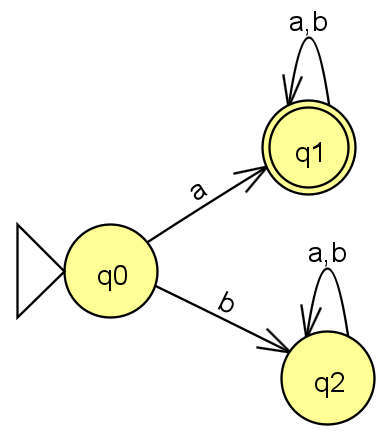
\includegraphics[width=0.2\textwidth]{../../../images/DFAs/ex1_q1.png}



% \vspace{3cm}
% \begin{flushleft}
% أرجو لكم وقتًا ممتعًا.

% الأستاذ محمود اغبارية.
% \end{flushleft}


% \end{document}


\ifwithsols
\title{حل ورقة تمرّن 9 - الحلقات المتداخلة}
\else
\title{ورقة تمرّن 9 - الحلقات المتداخلة}
\fi

\begin{document}

\maketitle
\thispagestyle{fancy}

\begin{enumerate}[itemsep=2em]

    \item
    ما هو ناتج مقطع الكود التالي؟
    \begin{boxCode}
    \begin{english}
    \begin{minted}{csharp}
for (int i = 1; i <= 2; i++)
{
    for (int j = 1; j <= 3; j++)
    {
        Console.Write("*");
    }
    Console.WriteLine();
}
    \end{minted}
    \end{english}
    \end{boxCode}
    \ifwithsols
    \begin{boxSolution}
    \begin{english}
    \begin{boxCode}
\begin{verbatim}
***
***
    \end{verbatim}
\end{boxCode}
    \end{english}
    \textbf{الشرح:} الحلقة الخارجية تدور مرتين (سطرين)، والحلقة الداخلية تطبع 3 نجوم في كل سطر.
    \end{boxSolution}
    \clearpage
    \fi

    \item
    كم مرة يطبع مقطع الكود التالي كلمة \textenglish{"Hello"}؟
    \begin{boxCode}
    \begin{english}
    \begin{minted}{csharp}
for (int i = 1; i <= 4; i++)
{
    for (int j = 1; j <= 3; j++)
    {
        Console.WriteLine("Hello");
    }
}
    \end{minted}
    \end{english}
    \end{boxCode}
    \ifwithsols
    \begin{boxSolution}
    \textbf{الجواب:} 12 مرة\\
    \textbf{الشرح:} $4 \times 3 = 12$ (الحلقة الخارجية 4 مرات × الحلقة الداخلية 3 مرات)
    \end{boxSolution}
    \fi

    \clearpage
    \item
    ما هو ناتج مقطع الكود التالي؟
    \begin{boxCode}
    \begin{english}
    \begin{minted}{csharp}
for (int i = 1; i <= 3; i++)
{
    for (int j = 1; j <= 2; j++)
    {
        Console.Write(i);
    }
    Console.WriteLine();
}
    \end{minted}
    \end{english}
    \end{boxCode}
    \ifwithsols
    \begin{boxSolution}
    \begin{english}
    \begin{boxCode}
\begin{verbatim}
11
22
33
    \end{verbatim}
\end{boxCode}
    \end{english}
    \textbf{الشرح:} في كل دورة للحلقة الخارجية، قيمة \textenglish{i} تطبع مرتين بسبب الحلقة الداخلية.
    \end{boxSolution}
    \clearpage
    \fi

        \item
    ما هو ناتج مقطع الكود التالي؟
    \begin{boxCode}
    \begin{english}
    \begin{minted}{csharp}
for (int i = 1; i <= 2; i++)
{
    for (int j = 1; j <= 3; j++)
    {
        Console.Write($"{i}{j} ");
    }
    Console.WriteLine();
}
    \end{minted}
    \end{english}
    \end{boxCode}
    \ifwithsols
    \begin{boxSolution}
    \begin{english}
    \begin{boxCode}
\begin{verbatim}
11 12 13
21 22 23
    \end{verbatim}
\end{boxCode}
    \end{english}
    \textbf{الشرح:} في كل دورة، يطبع رقم الصف (\textenglish{i}) مع رقم العمود (\textenglish{j}).
    \end{boxSolution}
    \fi

    \clearpage
    \item
    ما هو ناتج مقطع الكود التالي؟
    \begin{boxCode}
    \begin{english}
    \begin{minted}{csharp}
for (int i = 1; i <= 3; i++)
{
    for (int j = 1; j <= 4; j++)
    {
        Console.Write(j);
    }
    Console.WriteLine();
}
    \end{minted}
    \end{english}
    \end{boxCode}
    \ifwithsols
    \begin{boxSolution}
    \begin{english}
    \begin{boxCode}
\begin{verbatim}
1234
1234
1234
    \end{verbatim}
\end{boxCode}
    \end{english}
    \textbf{الشرح:} في كل دورة للحلقة الخارجية، الحلقة الداخلية تطبع 1234.
    \end{boxSolution}
    \clearpage
    \fi

    \item
    ما هي قيمة المتغير \textenglish{sum} في نهاية تنفيذ مقطع الكود التالي؟
    \begin{boxCode}
    \begin{english}
    \begin{minted}{csharp}
int sum = 0;
for (int i = 1; i <= 3; i++)
{
    for (int j = 1; j <= 2; j++)
    {
        sum += i;
    }
}
Console.WriteLine(sum);
    \end{minted}
    \end{english}
    \end{boxCode}
    \ifwithsols
    \begin{boxSolution}
    \textbf{الجواب:} 12\\
    \textbf{التتبع:}
    \begin{itemize}
        \item عندما \textenglish{i = 1}: يضاف 1 مرتين $\rightarrow$ \textenglish{sum = 2}
        \item عندما \textenglish{i = 2}: يضاف 2 مرتين $\rightarrow$ \textenglish{sum = 6}
        \item عندما \textenglish{i = 3}: يضاف 3 مرتين $\rightarrow$ \textenglish{sum = 12}
    \end{itemize}
    \end{boxSolution}
    \fi
\end{enumerate}

\clearpage
\begin{enumerate}[itemsep=2em]
    \item
    اكتب مقطع برنامج يستقبل من المستخدم طول مستطيل وعرضه ويطبع مستطيلاً من النجوم بالطول والعرض اللذين استقبلهما. \\
    مثلًا: إذا كان العرض 6 والطول 4 يكون هذا هو الناتج \\
    \begin{english}
    \begin{boxCode}
\begin{verbatim}
* * * * * *
* * * * * *
* * * * * *
* * * * * *
    \end{verbatim}
\end{boxCode}
    \end{english}
    \ifwithsols
    \begin{boxSolution}
    \begin{english}
    \begin{minted}{csharp}
for (int row = 1; row <= 4; row++)
{
    for (int col = 1; col <= 6; col++)
    {
        Console.Write("* ");
    }
    Console.WriteLine();
}
    \end{minted}
    \end{english}
    \end{boxSolution}
    \clearpage
    \fi

    \item
    اكتب مقطع برنامج يطبع مثلثاً من النجوم كالتالي:
    \begin{english}
    \begin{boxCode}
\begin{verbatim}
*
* *
* * *
* * * *
* * * * *
    \end{verbatim}
\end{boxCode}
    \end{english}
    \ifwithsols
    \begin{boxSolution}
    \begin{english}
    \begin{minted}{csharp}
for (int i = 1; i <= 5; i++)
{
    for (int j = 1; j <= i; j++)
    {
        Console.Write("* ");
    }
    Console.WriteLine();
}
    \end{minted}
    \end{english}
    \textbf{الشرح:} في كل سطر \textenglish{i}، نطبع \textenglish{i} نجوم.
    \end{boxSolution}
    \clearpage
    \fi

    \item
    اكتب مقطع برنامج يطبع الشكل التالي:
    \begin{english}
    \begin{boxCode}
\begin{verbatim}
1 1 1
2 2 2
3 3 3
4 4 4
    \end{verbatim}
\end{boxCode}
    \end{english}
    \ifwithsols
    \begin{boxSolution}
    \begin{english}
    \begin{minted}{csharp}
for (int i = 1; i <= 4; i++)
{
    for (int j = 1; j <= 3; j++)
    {
        Console.Write($"{i} ");
    }
    Console.WriteLine();
}
    \end{minted}
    \end{english}
    \end{boxSolution}
    \fi

    \clearpage
    \item
    اكتب مقطع برنامج يطبع الشكل التالي:
    \begin{english}
    \begin{boxCode}
\begin{verbatim}
*
* *
* * *
* *
*
    \end{verbatim}
\end{boxCode}
    \end{english}
    \begin{boxHint}
        ستحتاج إلى حلقتين منفصلتين - واحدة للجزء التصاعدي وأخرى للجزء التنازلي.
    \end{boxHint}
    \ifwithsols
    \begin{boxSolution}
    \begin{english}
    \begin{minted}{csharp}
for (int i = 1; i <= 3; i++)
{
    for (int j = 1; j <= i; j++)
    {
        Console.Write("* ");
    }
    Console.WriteLine();
}

for (int i = 2; i >= 1; i--)
{
    for (int j = 1; j <= i; j++)
    {
        Console.Write("* ");
    }
    Console.WriteLine();
}
    \end{minted}
    \end{english}
    \end{boxSolution}
    \fi

\end{enumerate}

\end{document}
